This chapter will provide a comprehensive overview of the technical foundations essential to the project. It begins with an in-depth exploration of virtualization and Oracle Linux, detailing its core characteristics and key features. Following this, the chapter delves into the Unbreakable Enterprise Kernel (UEK) and its significance. The discussion then extends to the roles and functionalities of QEMU and Libvirt tools. The chapter concludes by outlining the project requirements, specifying the necessary features and criteria to achieve the project’s objectives.

\newpage
\fancyhead[R]{\textsc{Chapter 2 - Technical Foundations and Project Essentials}}
\hypertarget{secondchapter}{}
\section{Technical Background}

%% Virtualization
\subsection{Virtualization}
Virtualization serves as a cornerstone technology in modern IT infrastructure, enabling a single physical machine, or VM Host Server, to run multiple operating systems simultaneously as virtual machines (VM Guests). This approach abstracts the underlying hardware resources, creating isolated environments where each operating system can function independently, as though it were on dedicated hardware.

%% Mechanisms of Virtualization
\subsubsection[Mechanisms of Virtualization]{Mechanisms of Virtualization}
The critical enabler of virtualization is the hypervisor, a software layer that directly interfaces with the hardware of the VM Host Server. The hypervisor manages the allocation of resources such as CPU, memory, and storage, distributing them among the various VM Guests. By presenting each guest with a virtualized hardware interface, the hypervisor ensures that multiple operating systems can coexist without interference. There are two primary types of hypervisors utilized in enterprise environments: Type 1 (bare-metal hypervisors) and Type 2 (hosted hypervisors).
\begin{center}
    \centering
    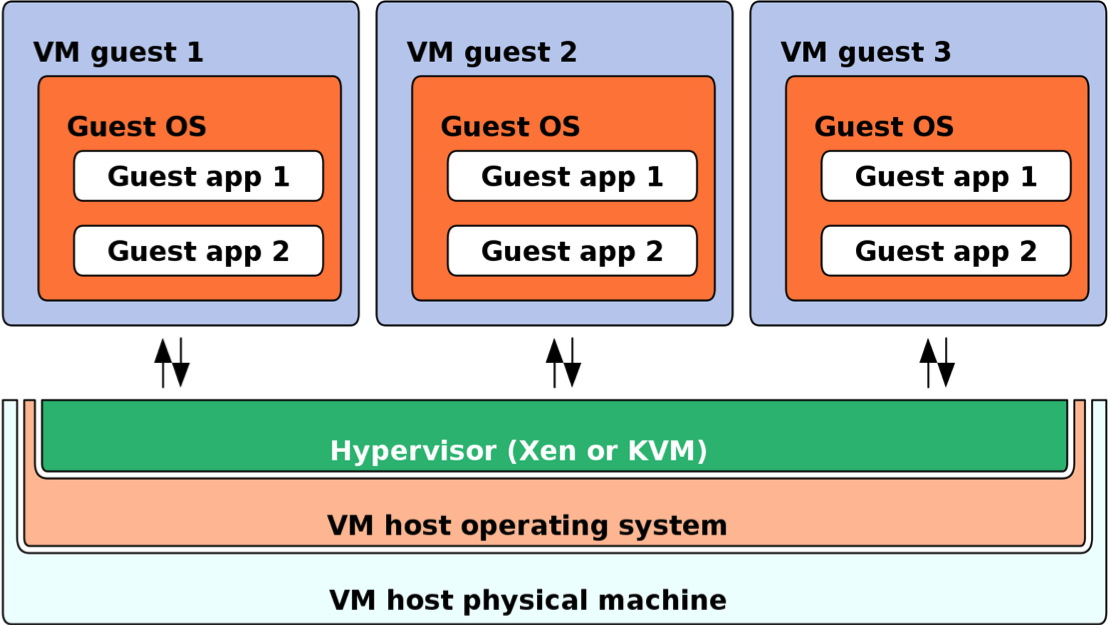
\includegraphics[width=1\textwidth]{Images/VirtualizationSchema.png}
    \captionof{figure}{General Schema of Virtualization} \cite{Source}
    \label{fig:source}
\end{center}

%% Advantages of Virtualization in Cloud Infrastructure
\subsubsection[Advantages of Virtualization in Cloud Infrastructure]{Advantages of Virtualization in Cloud Infrastructure}
In the context of Oracle Cloud Infrastructure (OCI), virtualization provides several strategic advantages:\mynewline
\begin{itemize}
    \item \textbf{Cost Optimization:} Virtualization reduces the need for additional hardware by allowing multiple operating systems to run on a single physical server, leading to significant savings in hardware, power, and cooling costs;
    \item \textbf{Enhanced Resource Utilization:} By maximizing the use of available resources, virtualization helps ensure that CPU, memory, and storage are used efficiently, reducing waste and improving overall system performance;
    \item \textbf{Operational Flexibility:} Virtualization facilitates rapid provisioning and deployment of virtual machines, enabling IT teams to quickly respond to changing business needs. Features such as live migration and snapshots further enhance the flexibility and resilience of virtualized environments;
    \item \textbf{Disaster Recovery and Business Continuity:} Virtualization supports advanced disaster recovery strategies by enabling features like VM snapshots, live migration, and automated failover, which are critical for maintaining business continuity in the event of hardware failures or other disruptions.
\end{itemize}

%% Virtualization Modes
\subsubsection[Virtualization Modes]{Virtualization Modes}
\begin{itemize}
    \item \textbf{Full Virtualization:} This mode emulates complete hardware, allowing unmodified operating systems to run in a virtualized environment. It is particularly useful when running legacy applications that require full emulation of underlying hardware;
    \item \textbf{Paravirtualization:} In this mode, the guest operating system is modified to interact directly with the hypervisor, leading to improved performance. Paravirtualization is advantageous in scenarios where high efficiency and performance are required;
    \item \textbf{Hardware-Assisted Virtualization (HVM):} This mode leverages hardware features such as Intel VT-x and AMD-V to enhance virtualization performance. HVM combines the compatibility of full virtualization with the efficiency of paravirtualization, making it ideal for high-performance computing environments.
\end{itemize}


%% Oracle Linux
\subsection{Oracle Linux}
Oracle Linux, often abbreviated as OL (previously known as Oracle Enterprise Linux or OEL), is a robust and versatile Linux distribution developed and freely distributed by Oracle Corporation. Since its initial release in 2006, Oracle Linux has been partially licensed under the GNU General Public License (GPL), making it an open-source platform. It is built using the source code from Red Hat Enterprise Linux (RHEL), with Oracle replacing Red Hat's branding with its own. This distribution plays a significant role in Oracle's ecosystem, serving as the foundation for Oracle Cloud Infrastructure (OCI) and Oracle Engineered Systems, including Oracle Exadata.
\begin{center}
    \centering
    
\includegraphics[width=0.3\textwidth]{Images/Oracle Linux.png}
    \captionof{figure}{ Oracle Linux Logo} \cite{OL-logo}
    \label{fig:walt}
\end{center}

%% Compatibility with Red Hat Enterprise Linux (RHEL)
\subsubsection[Compatibility with Red Hat Enterprise Linux (RHEL)]{Compatibility with Red Hat Enterprise Linux (RHEL)}
Oracle Linux is designed to maintain binary compatibility with RHEL, ensuring that applications developed for RHEL can run seamlessly on Oracle Linux without modification. Oracle offers two kernel options within Oracle Linux:
\begin{itemize}
    \item \textbf{Red Hat Compatible Kernel (RHCK):} This kernel is identical to the one provided by RHEL, offering users a stable and reliable environment that is fully compatible with the RHEL ecosystem;
    \item \textbf{Unbreakable Enterprise Kernel (UEK):} UEK is Oracle's optimized Linux kernel, tailored for high-performance environments. It enhances areas like OLTP, InfiniBand, and SSD access, and supports advanced features such as RDS, asynchronous I/O, and Btrfs. Since this kernel is used in our project, we will provide further details in the next sections.
\end{itemize}

Oracle’s commitment to maintaining compatibility with RHEL allows enterprises to leverage the stability of RHEL while benefiting from Oracle’s additional enhancements, particularly when using Oracle's hardware and cloud solutions.

%% Virtualization Support
\subsubsection[Virtualization Support]{Virtualization Support}
Oracle Linux is fully equipped to support modern virtualization needs, offering the KVM hypervisor as part of its distribution. Additionally, it includes an oVirt-based management tool, which provides a robust interface for managing virtualized environments. Oracle Linux also supports other popular virtualization platforms, such as VMware and Oracle VM, which is based on the Xen hypervisor.


%% UEK
\subsection{Unbreakable Enterprise Kernel (UEK)}
The Unbreakable Enterprise Kernel (UEK) is a high-performance Linux kernel developed by Oracle, tailored specifically for enterprise-level workloads and Oracle environments. Designed to prioritize stability and efficiency, UEK closely follows the mainline Linux kernel while integrating Oracle’s enhancements. It is extensively tested and is the recommended kernel for Oracle’s Engineered Systems, Oracle Cloud Infrastructure, and other large-scale enterprise deployments.

%% Capabilities and Features
\subsubsection[Capabilities and Features]{Capabilities and Features}
UEK offers a range of advanced capabilities, making it particularly suitable for demanding enterprise applications.  It incorporates a multitude of advanced features, such as:
\begin{itemize}
    \item \textbf{Performance:} Engineered for Oracle workloads, UEK enhances the performance of databases and applications through optimized task scheduling, low-latency networking, and advanced memory management techniques;
    \item \textbf{Security:} It strengthens system protection with the latest security features and patches, including support for Security-Enhanced Linux (SELinux), control groups (cgroups), and other security-enhancing mechanisms;
    \item \textbf{Virtualization:} UEK supports modern virtualization technologies like KVM and Xen, offering paravirtualized drivers, optimized memory management, and advanced network and storage virtualization to maximize virtualization infrastructure efficiency;
    \item \textbf{Hardware Support:} Tailored for Oracle hardware, UEK includes support for cutting-edge technologies such as Intel Xeon Scalable processors and NVMe SSDs, as well as advanced features like NUMA and CPU hot-plugging to optimize hardware resource utilization;
    \item \textbf{Open Source:} As an open-source kernel, UEK is fully compatible with the Linux kernel and can be used across other Linux distributions, promoting transparency and flexibility in its deployment.
\end{itemize}

%% Key Versions: UEK7U2 and UEK6U3
\subsubsection[Key Versions: UEK7U2 and UEK6U3]{Key Versions: UEK7U2 and UEK6U3}
Oracle's Unbreakable Enterprise Kernel continues to evolve with each release, bringing new features and optimizations. Two significant updates are used in this project : UEK7U2 and UEK6U3, each offering unique enhancements:
\begin{itemize}
    \item \textbf{UEK7U2:} The second update of UEK7 introduces further improvements in performance and security, specifically designed for Oracle's cloud and on-premises environments. This update enhances support for the latest hardware, including next-generation processors and storage technologies. UEK7U2 also introduces refined scheduling algorithms and networking optimizations, making it an ideal choice for workloads that demand low latency and high throughput;
    \item \textbf{UEK6U3:} Update 3 in the UEK6 series builds on previous stability and performance enhancements. It focuses on extended hardware compatibility, especially for older Oracle systems, and includes critical security patches. This update is optimized for environments where reliability and backward compatibility are crucial, ensuring legacy applications run smoothly without sacrificing performance.
\end{itemize}

These updates underline Oracle's commitment to providing a flexible and high-performing kernel tailored to the evolving needs of enterprise environments.

%% QEMU
\subsection{QEMU}
QEMU (Quick Emulator) is an open-source machine emulator and virtualizer that provides a comprehensive platform for hardware virtualization. As a crucial component in many virtualization environments, QEMU facilitates the creation and management of virtual machines by emulating hardware components and providing a range of virtual hardware devices.

%% Modes of Operation and Integration
\subsubsection[Modes of Operation and Integration]{Modes of Operation and Integration}
QEMU can operate in two primary modes: full system emulation and user-mode emulation. In full system emulation mode, QEMU emulates an entire computer system, including CPU, memory, and peripheral devices, allowing users to run an entire operating system as if it were on physical hardware. In user-mode emulation, QEMU enables running applications compiled for different processor architectures on a host system, effectively providing cross-platform compatibility.\mynewline

QEMU integrates seamlessly with various hypervisors and virtualization management tools, such as KVM (Kernel-based Virtual Machine) and Libvirt. When used in conjunction with KVM, QEMU leverages hardware acceleration features to enhance performance, delivering near-native execution speeds for virtualized environments.


%% Capabilities and Features
\subsubsection[Capabilities and Features]{Capabilities and Features}
QEMU provides a diverse array of features that contribute to its versatility and effectiveness in virtualization:
\begin{itemize}
\item \textbf{Hardware Emulation:} Supports a wide range of hardware devices and peripherals, including CPUs, memory, storage controllers, and network interfaces, allowing users to create virtual machines with diverse configurations;
\item \textbf{Virtualization Acceleration:} When paired with KVM, QEMU utilizes hardware acceleration technologies like Intel VT-x and AMD-V to enhance the performance of virtual machines, providing near-native execution speeds;
\item \textbf{Live Migration:} Facilitates the movement of running virtual machines between physical hosts with minimal downtime, supporting continuous availability and load balancing;
\item \textbf{Snapshot and Checkpoints:} Enables the creation of snapshots and checkpoints of virtual machines, allowing users to save and restore the state of a VM at any point in time, which is valuable for testing and disaster recovery;
\item \textbf{Cross-Platform Compatibility:} Offers support for multiple processor architectures and operating systems, making it a flexible tool for diverse virtualization scenarios;
\item \textbf{Customizable Devices:} Provides the ability to define and configure various virtual devices, including graphics cards, network adapters, and storage controllers, to tailor virtual machines to specific needs.
\end{itemize}

%% Libvirt
\subsection{Libvirt}

Libvirt is a comprehensive suite of software that provides a unified API (Application Programming Interface) for managing a variety of virtualization solutions, including KVM, QEMU, Xen, Virtuozzo, VMware ESX, and others. This suite comprises an API library, the system service libvirtd, and a command-line utility known as virsh. The modular design of libvirt facilitates extending its functionality, making it a versatile tool for managing virtual environments.

%% Libvirt Architecture
\subsubsection[Libvirt Architecture]{Libvirt Architecture}
The libvirtd service operates on the virtual machine (VM) host, handling interactions between the host's configuration and the virtual environments it supports. Client libraries and utilities connect to libvirtd to gather configuration data and resource information for the host servers. Each virtual machine's configuration is managed through XML files, which can be manipulated using various methods.
Libvirt supports both command-line and graphical user interface (GUI) tools for managing virtual machines. For command-line management, virsh provides a robust tool for configuring and controlling VMs, while virt-manager offers a graphical interface for those who prefer visual management. Additionally, other utilities like virt-install, virt-clone, and virt-image assist in creating, cloning, and managing virtual machines and their disks.
\begin{center}
    \centering
    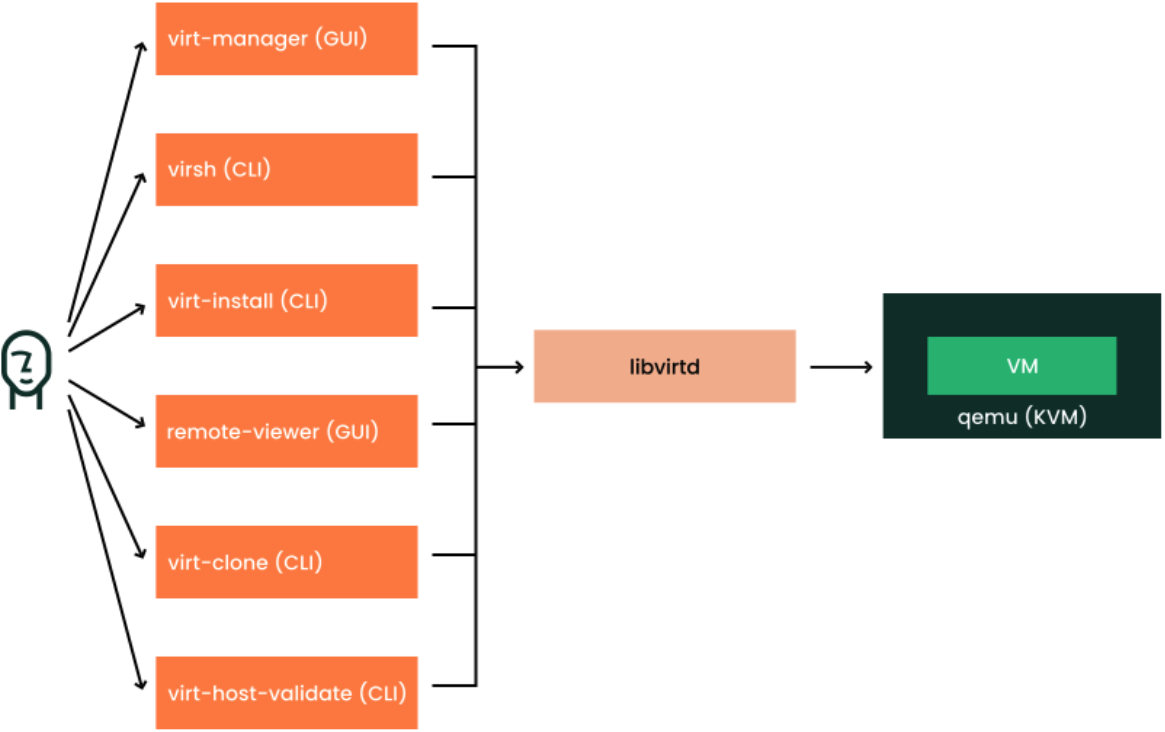
\includegraphics[width=1\textwidth]{Images/Libvirt Overview.png}
    \captionof{figure}{Libvirt Overview} \cite{Libvirt}
    \label{fig:libvirt}
\end{center}
\noindent
\mynewline

%% Benefits of Using Libvirt
\subsubsection[Benefits of Using Libvirt]{Benefits of Using Libvirt}
Libvirt provides several advantages that enhance the management and operation of virtual environments:
\begin{itemize}
    \item \textbf{Basic Monitoring:} Allows for monitoring of both host systems and virtual machines, providing essential insights into their status and performance;
    \item \textbf{Automation and Scripting:} Facilitates automation of complex virtualization tasks and workflows through scripting, streamlining management processes;
    \item \textbf{Remote Management:} Enables remote management of virtualization hosts over secure protocols such as SSH, which is crucial for managing resources on remote servers;
    \item \textbf{Headless Server Management:} Offers management capabilities for headless servers that lack a graphical interface, using command-line tools as the primary method of control;
    \item \textbf{Custom Reporting:} Supports scripting and commands for generating custom reports, providing flexibility in monitoring and documentation;
    \item \textbf{Multi-Hypervisor Support:} Provides a unified tool for managing multiple hypervisors, ensuring compatibility and efficiency across different virtualization technologies.
\end{itemize}

By integrating libvirt into virtualization strategies, organizations can achieve greater control, efficiency, and flexibility in managing their virtual environments.

%% Project Requirement
\section{Project Requirements}
Defining the project requirements is crucial to outline the expected outcomes and objectives clearly. The following are the main requirements to be addressed:

\begin{itemize}
    \item \textbf{Validation of Functionality:} Ensure proper operation of QEMU and Libvirt across various Oracle Linux versions, including components like UEK, Libiscsi, and OVMF;
    \item \textbf{Regression Testing:} Detect and address any regressions or issues introduced by new software updates;
    \item \textbf{Compatibility Testing:} Verify interoperability of different QEMU and Libvirt versions with diverse host and guest OS configurations;
    \item \textbf{Performance Assessment:} Monitor and document the performance of virtualization modules to ensure they meet established standards;
    \item \textbf{Documentation:} Provide comprehensive reports on the testing procedures, results, and any issues encountered or resolved.
\end{itemize}
\section{Conclusion}
This chapter has delivered a thorough analysis of the technical aspects critical to the project. It started with an overview of virtualization and Oracle Linux, followed by a detailed look at the Unbreakable Enterprise Kernel and its features. The discussion then covered QEMU’s modes of operation and integration, and examined the architecture and benefits of Libvirt. The chapter concluded by defining the project requirements necessary for meeting our goals.